\documentclass[../../main.tex]{subfiles}

\graphicspath{{../../image/}{../../figure/}}

\begin{document}

\section{基本采样}\label{section:ch14-基本采样}

在本节中，我们将介绍一系列相对简单的采样策略，用于从给定分布中生成随机样本。由于样本是由计算机算法生成的，它们是伪随机（pseudo-random）的，也就是说，它们将使用确定性算法来运算，但仍必须通过适当的随机性测试。这里我们假设已经存在一个确定性算法，它能生成在 $(0,1)$ 区间上均匀分布的伪随机数，事实上，大多数软件平台都内置了这样的功能。

\subsection{期望}\label{subsection:ch14-期望}

虽然在某些应用中我们可以直接使用样本本身，但在更多情况下，我们的目标是计算某个概率分布的期望。假设我们希望找到函数 $f(\bm{z})$ 关于概率分布 $p(\bm{z})$ 的期望。在这里，$\bm{z}$ 的分量可能包括离散变量、连续变量或它们两者的组合。对于连续变量，期望定义为
\begin{align}
\mathbb{E}[f]=\int f(\bm{z})\,p(\bm{z})\,\mathrm{d}\bm{z},
\label{align:ch14-期望定义}
\end{align}
其中，积分在离散变量的情况下被求和替代。\cref{figure:ch14-期望示意}展示了单个连续变量的情况。

我们在此假设这样的期望过于复杂，无法使用解析方法准确计算，这时候就需要用采样方法近似计算。采样方法的基本思路是获得从分布 $p(\bm{z})$ 中独立地抽取的一组样本 $\bm{z}^{(l)}$（其中 $l=1,\cdots,L$），使得期望\eqref{align:ch14-期望定义}可以通过有限和的形式来近似：
\begin{align}
\overline{f}=\frac{1}{L}\sum_{l=1}^{L}f\!\left(\bm{z}^{(l)}\right).
\label{align:ch14-mc估计}
\end{align}

\begin{figure}[htbp]
\centering
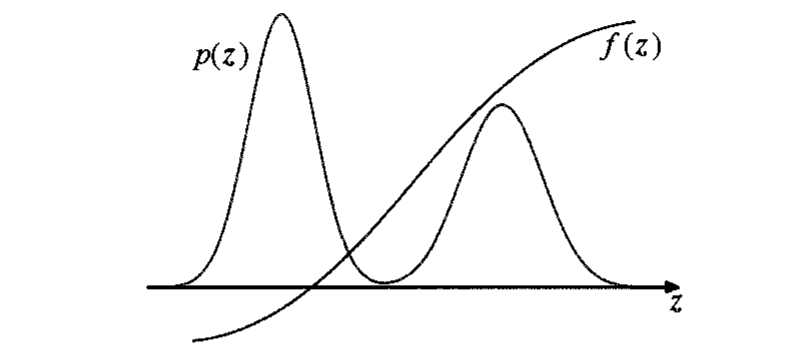
\includegraphics[width=0.52\textwidth]{ch14-fig14.1-expectation.png}
\caption{一个函数 $f(z)$，我们需要计算它关于概率分布 $p(z)$ 的期望（示意图）}
\label{figure:ch14-期望示意}
\end{figure}

如果样本 $\bm{z}^{(l)}$ 是从概率分布 $p(\bm{z})$ 中抽取的，则 $\mathbb{E}[\overline{f}]=\mathbb{E}[f(\bm{z})]$，因此估计量 $\overline{f}$ 具有正确的均值（见\cref{exercise:ch14-01}）。

\begin{proposition}[Monte Carlo 估计的无偏性]\label{proposition:ch14-mc无偏性}
设 $\bm{z}^{(1)},\cdots,\bm{z}^{(L)}$ 的边缘分布均为 $p(\bm{z})$，且 $\mathbb{E}\left[\left|f(\bm{z})\right|\right]<\infty$。则由\eqref{align:ch14-mc估计}定义的估计量 $\overline{f}$ 是 $\mathbb{E}[f(\bm{z})]$ 的无偏估计，即 $\mathbb{E}[\overline{f}]=\mathbb{E}[f(\bm{z})]$。
\end{proposition}

\begin{proof}
由\eqref{align:ch14-mc估计}与期望的线性性，
\begin{align*}
\mathbb{E}\left[\overline{f}\right]=\mathbb{E}\left[\frac{1}{L}\sum_{l=1}^{L}f\!\left(\bm{z}^{(l)}\right)\right]=\frac{1}{L}\sum_{l=1}^{L}\mathbb{E}\left[f\!\left(\bm{z}^{(l)}\right)\right]=\frac{1}{L}\sum_{l=1}^{L}\mathbb{E}[f(\bm{z})]=\mathbb{E}[f(\bm{z})].
\end{align*}
上面的推导只用到每个 $\bm{z}^{(l)}$ 的边缘分布为 $p(\bm{z})$，并未用到样本之间的独立性。
\end{proof}

% SUPPLEMENT: parent=proposition:ch14-mc无偏性; kind=motivation; location=紧随其后的 remark（重构新增）
\begin{remark}（重构新增）本命题说明了 Monte Carlo 估计「至少不会系统性地偏离真值」，这是把有限和当作积分使用的全部依据。条件 $\mathbb{E}[|f(\bm{z})|]<\infty$ 不可省：若该期望不存在（例如重尾情形），则 $\mathbb{E}[\overline{f}]$ 本身没有定义，无偏性也就无从谈起；此时中心极限定理同样失效，样本均值不再收敛。值得注意的是，命题只要求各样本的边缘分布相同而不要求独立，因此它对 Markov 链产生的相关样本仍然成立（见\cref{section:ch14-mcmc}）；独立性只在控制方差时起作用，见\cref{proposition:ch14-mc方差}。此外，$\overline{f}$ 的分子是 $L$ 项之和，故无偏性依赖于权重 $1/L$ 的精确取值；若改用依赖样本的自适应权重，无偏性需要另行证明。
\end{remark}

我们也可以把它改成
\begin{align}
\mathbb{E}[f(\bm{z})]\simeq\frac{1}{L}\sum_{l=1}^{L}f\!\left(\bm{z}^{(l)}\right),
\label{align:ch14-无偏近似}
\end{align}
其中符号 $\simeq$ 表示右侧是左侧的无偏估计量，也就是说，当对噪声分布进行平均时，两侧是相等的（见\cref{exercise:ch14-01}）。估计量\eqref{align:ch14-mc估计}的方差由下式给出：
\begin{align}
\operatorname{var}\left[\overline{f}\right]=\frac{1}{L}\,\mathbb{E}\left[\left(f(\bm{z})-\mathbb{E}[f(\bm{z})]\right)^{2}\right].
\label{align:ch14-估计方差}
\end{align}

\begin{proposition}[Monte Carlo 估计的方差]\label{proposition:ch14-mc方差}
在\cref{proposition:ch14-mc无偏性}的条件下，若进一步假设 $\bm{z}^{(1)},\cdots,\bm{z}^{(L)}$ 相互独立，且 $\operatorname{var}[f(\bm{z})]<\infty$，则\eqref{align:ch14-估计方差}成立，即
\begin{align}
\operatorname{var}\left[\overline{f}\right]=\frac{1}{L}\operatorname{var}[f(\bm{z})].
\label{align:ch14-方差iid}
\end{align}
\end{proposition}

\begin{proof}
记 $\sigma^{2}=\operatorname{var}[f(\bm{z})]=\mathbb{E}\left[\left(f(\bm{z})-\mathbb{E}[f(\bm{z})]\right)^{2}\right]$。由独立性，各 $f(\bm{z}^{(l)})$ 相互独立且方差同为 $\sigma^{2}$，于是
\begin{align*}
\operatorname{var}\left[\overline{f}\right]=\operatorname{var}\left[\frac{1}{L}\sum_{l=1}^{L}f\!\left(\bm{z}^{(l)}\right)\right]=\frac{1}{L^{2}}\sum_{l=1}^{L}\operatorname{var}\left[f\!\left(\bm{z}^{(l)}\right)\right]=\frac{1}{L^{2}}\cdot L\sigma^{2}=\frac{\sigma^{2}}{L},
\end{align*}
这正是\eqref{align:ch14-估计方差}与\eqref{align:ch14-方差iid}的右端。
\end{proof}

% SUPPLEMENT: parent=proposition:ch14-mc方差; kind=motivation; location=紧随其后的 remark（重构新增）
\begin{remark}（重构新增）本命题给出了 Monte Carlo 方法最核心的定量结论：误差的平方按 $1/L$ 衰减，即标准差按 $1/\sqrt{L}$ 衰减，而且这一速率\emph{与 $\bm{z}$ 的维数无关}——这正是采样方法在高维问题中优于网格求和的原因。两个条件各有作用：独立性保证了交叉项 $\operatorname{cov}[f(\bm{z}^{(l)}),f(\bm{z}^{(l')})]$ 全部为零，若样本相关（例如 MCMC 的相邻状态），则
\begin{align*}
\operatorname{var}\left[\overline{f}\right]=\frac{\sigma^{2}}{L}\left(1+2\sum_{k\geqslant1}\rho_k\right),
\end{align*}
其中 $\rho_k$ 为滞后 $k$ 的自相关系数，有效样本量按因子 $\left(1+2\sum_k\rho_k\right)$ 缩小，这就是\cref{section:ch14-mcmc}中「丢弃大部分序列、只保留每第 $M$ 个样本」做法的依据；有限方差则保证 $\sigma^{2}$ 存在，否则 $1/L$ 的速率不再成立。最后提醒，方差小并不等于估计准确：若 $f$ 在 $p$ 的高密度区取值很小而在低密度区取值很大，则 $\sigma^{2}$ 会很大，仍需要很大的 $L$ 才能达到所需精度。
\end{remark}

该方差是函数 $f(\bm{z})$ 在概率分布 $p(\bm{z})$ 下的方差。注意，这种方差会随着 $L$ 的增加而线性减小，并且不依赖于 $\bm{z}$ 的维度，从原则上讲，使用相对较小的样本集合 $\left\{\bm{z}^{(l)}\right\}$ 就有可能获得高精度。然而，问题在于样本集合 $\left\{\bm{z}^{(l)}\right\}$ 中的样本可能不是独立的，所以有效样本量可能比表面上的样本量要小得多。另外，在\cref{figure:ch14-期望示意}中，如果 $f(\bm{z})$ 在 $p(\bm{z})$ 较大的区域很小，在 $p(\bm{z})$ 较小的地方反而很大，则期望可能被小概率区域主导，这意味着为了达到足够的准确度，可能需要较大的样本量。

\subsection{标准分布}\label{subsection:ch14-标准分布}

现在假设我们已经有了一个均匀分布随机数的来源，我们讨论如何从简单的非均匀分布中生成随机数。假设 $z$ 在区间 $(0,1)$ 上均匀分布，并且我们使用某个函数 $g(\cdot)$ 来变换 $z$ 的值，使得 $y=g(z)$。$y$ 的分布将由下式决定：
\begin{align}
p(y)=p(z)\left|\frac{\mathrm{d}z}{\mathrm{d}y}\right|,
\label{align:ch14-变量变换}
\end{align}
在这里，$p(z)=1$。我们的目标是选择合适的函数 $g(\cdot)$，让生成的 $y$ 具有某个特定的期望分布 $p(y)$。对\eqref{align:ch14-变量变换}进行积分，可以得到
\begin{align}
z=\int_{-\infty}^{y}p(\hat{y})\,\mathrm{d}\hat{y}\equiv h(y),
\label{align:ch14-累积分布变换}
\end{align}
这是 $p(y)$ 的不定积分。$y=h^{-1}(z)$，所以我们需要使用一个变换函数，该函数是目标分布不定积分的反函数，如\cref{figure:ch14-变换方法}所示。

\begin{figure}[htbp]
\centering
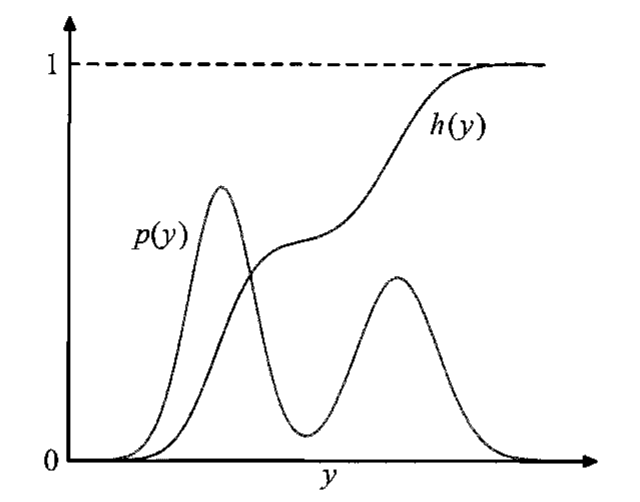
\includegraphics[width=0.45\textwidth]{ch14-fig14.2-transform.png}
\caption{生成非均匀分布随机数的变换方法的几何解释。$h(y)$ 是期望的目标分布 $p(y)$ 的不定积分。如果用 $y=h^{-1}(z)$ 变换均匀分布的随机变量 $z$，那么得到的变量 $y$ 将服从 $p(y)$ 分布}
\label{figure:ch14-变换方法}
\end{figure}

\begin{definition}[逆变换采样]\label{definition:ch14-逆变换采样}
设目标分布 $p(y)$ 的累积分布函数为 $h(y)=\int_{-\infty}^{y}p(\hat{y})\,\mathrm{d}\hat{y}$，且 $h$ 严格单调递增。若 $z$ 服从区间 $(0,1)$ 上的均匀分布，则称由
\begin{align*}
y=h^{-1}(z)
\end{align*}
生成样本的方法为逆变换采样（inverse transform sampling）。
\end{definition}

% SUPPLEMENT: parent=definition:ch14-逆变换采样; kind=motivation; location=紧随其后的 remark（重构新增）
\begin{remark}（重构新增）逆变换采样的动机是：均匀分布是最容易生成的分布，而累积分布函数 $h$ 恰好把任意分布「压平」成均匀分布——$h(y)\sim\mathcal{U}(0,1)$，于是把这一过程反过来，就能把均匀随机数「拉伸」成目标分布。定义中的两个条件都不可省：单调性保证 $h^{-1}$ 存在且唯一（若 $p$ 有零密度区间，$h$ 只能做到单调不减，此时需在平台上取广义逆 $h^{-1}(z)=\inf\{y:h(y)\geqslant z\}$，结论仍然成立）；$(0,1)$ 上的均匀性保证 $P(z\leqslant h(y))=h(y)$。定义并不要求 $p$ 归一化常数已知，但要求能对 $p$ 积分并求反函数，这一要求把方法限制在少数解析可积的分布上——这正是本节随后转向拒绝采样与重要性采样的原因。
\end{remark}

\begin{proposition}[逆变换采样的正确性]\label{proposition:ch14-逆变换正确性}
设 $p(y)$ 为概率密度，$h(y)=\int_{-\infty}^{y}p(\hat{y})\,\mathrm{d}\hat{y}$ 严格单调递增且连续，$z\sim\mathcal{U}(0,1)$，$y=h^{-1}(z)$。则 $y$ 的密度函数恰为 $p(y)$。
\end{proposition}

\begin{proof}
任取 $y_0\in\mathbb{R}$。由 $h$ 严格单调递增，$h^{-1}(z)\leqslant y_0$ 与 $z\leqslant h(y_0)$ 等价，于是
\begin{align*}
P(y\leqslant y_0)=P\left(h^{-1}(z)\leqslant y_0\right)=P\left(z\leqslant h(y_0)\right)=h(y_0)=\int_{-\infty}^{y_0}p(\hat{y})\,\mathrm{d}\hat{y},
\end{align*}
这里用到 $z$ 在 $(0,1)$ 上均匀分布且 $h(y_0)\in(0,1)$。上式右端关于 $y_0$ 可微且导数为 $p(y_0)$，故 $y$ 的累积分布函数是 $p$ 的不定积分，$y$ 的密度为 $p(y)$。
\end{proof}

% SUPPLEMENT: parent=proposition:ch14-逆变换正确性; kind=motivation; location=紧随其后的 remark（重构新增）
\begin{remark}（重构新增）证明的关键一步是把「$y$ 的分布」转化为「$z$ 的分布」：由于 $h^{-1}$ 单调，事件 $\{h^{-1}(z)\leqslant y_0\}$ 与 $\{z\leqslant h(y_0)\}$ 完全相同，而后者在均匀分布下的概率就是区间长度 $h(y_0)$。这解释了为什么\eqref{align:ch14-累积分布变换}中的下限取 $-\infty$：$h$ 必须是\emph{完整的}累积分布函数，才能把 $(0,1)$ 映满。若只取不定积分的某一个原函数 $H(y)+C$，则 $z$ 的取值范围不再是 $(0,1)$，必须先用 $H$ 的上下确界做仿射归一并相应修改反函数。条件「$h$ 连续」保证 $p$ 没有原子，否则 $h$ 有跳跃，$h^{-1}$ 在跳跃区间上不唯一，但按广义逆取值时结论不变。
\end{remark}

以指数分布为例
\begin{align}
p(y)=\lambda\exp(-\lambda y),\qquad 0\leqslant y<\infty.
\label{align:ch14-指数分布}
\end{align}
在这种情况下，\eqref{align:ch14-累积分布变换}中的积分的下限是 $0$，因此 $h(y)=1-\exp(-\lambda y)$。如果我们使用 $y=-\lambda^{-1}\ln(1-z)$ 变换均匀分布的随机变量 $z$，那么 $y$ 将服从指数分布。

\begin{example}[ 指数分布的逆变换采样]\label{example:ch14-指数分布采样}
设 $z\sim\mathcal{U}(0,1)$，令
\begin{align*}
y=-\frac{1}{\lambda}\ln(1-z),\qquad \lambda>0.
\end{align*}
验证 $y$ 服从\eqref{align:ch14-指数分布}给出的指数分布。
\end{example}

\begin{solution}（重构新增）由\eqref{align:ch14-指数分布}，$h(y)=\int_{0}^{y}\lambda e^{-\lambda \hat{y}}\,\mathrm{d}\hat{y}=1-e^{-\lambda y}$，它在 $[0,\infty)$ 上严格递增，值域为 $[0,1)$。解 $z=1-e^{-\lambda y}$ 得 $y=-\lambda^{-1}\ln(1-z)$，与题设一致；又 $1-z$ 与 $z$ 同为 $(0,1)$ 上的均匀随机变量，故也可写 $y=-\lambda^{-1}\ln z$。由\cref{proposition:ch14-逆变换正确性}，$y$ 的密度为 $p(y)=\lambda e^{-\lambda y}$（$y\geqslant 0$）。这里 $h$ 的值域为 $[0,1)$ 而 $z\in(0,1)$，端点 $z=0$ 的概率为零，不影响分布。
\end{solution}

可以应用变量变换方法的另一种分布是 Cauchy 分布：
\begin{align}
p(y)=\frac{1}{\pi}\frac{1}{1+y^{2}}.
\label{align:ch14-cauchy分布}
\end{align}
在这种情况下，不定积分的反函数可以用正切函数表示（见\cref{exercise:ch14-04}）。

\begin{example}[ Cauchy 分布的逆变换采样]\label{example:ch14-cauchy分布采样}
设 $z\sim\mathcal{U}(0,1)$，求变换 $y=f(z)$，使 $y$ 服从\eqref{align:ch14-cauchy分布}给出的 Cauchy 分布。
\end{example}

\begin{solution}（重构新增）由\eqref{align:ch14-cauchy分布}，
\begin{align*}
h(y)=\int_{-\infty}^{y}\frac{1}{\pi}\frac{1}{1+\hat{y}^{2}}\,\mathrm{d}\hat{y}=\frac{1}{\pi}\arctan y+\frac{1}{2},
\end{align*}
其值域为 $(0,1)$ 且严格递增。令 $z=\frac{1}{\pi}\arctan y+\frac{1}{2}$，解得 $y=\tan\left(\pi\left(z-\frac{1}{2}\right)\right)$。由\cref{proposition:ch14-逆变换正确性}，该 $y$ 的密度为\eqref{align:ch14-cauchy分布}。Cauchy 分布没有有限的期望与方差，这提醒我们\cref{proposition:ch14-mc方差}中的有限方差条件是实质性的。
\end{solution}

将该方法推广到多元变量的情形，需要引入变量变换的Jacobi行列式，于是有
\begin{align}
p(y_{1},\cdots,y_{M})=p(z_{1},\cdots,z_{M})\left|\frac{\partial(z_{1},\cdots,z_{M})}{\partial(y_{1},\cdots,y_{M})}\right|.
\label{align:ch14-多元变量变换}
\end{align}

作为变换方法的最后一个例子，我们介绍用于生成 Gauss 分布样本的 Box-Muller 方法。首先，我们生成一对均匀分布的随机数 $z_{1},z_{2}\in(-1,1)$，这可以通过对在区间 $(0,1)$ 上均匀分布的变量 $z$ 进行 $z\rightarrow 2z-1$ 线性变换来实现。接下来丢弃所有不满足条件 $z_{1}^{2}+z_{2}^{2}\leqslant 1$ 的数对，这将产生一个在单位圆内均匀分布的点集，且其概率密度为 $p(z_{1},z_{2})=1/\pi$，如\cref{figure:ch14-box-muller}所示。

最后，对于每对 $z_{1},z_{2}$，我们计算量
\begin{align}
y_{1}&=z_{1}\left(\frac{-2\ln r^{2}}{r^{2}}\right)^{1/2},
\label{align:ch14-box-muller-y1}\\
y_{2}&=z_{2}\left(\frac{-2\ln r^{2}}{r^{2}}\right)^{1/2},
\label{align:ch14-box-muller-y2}
\end{align}
其中 $r^{2}=z_{1}^{2}+z_{2}^{2}$（见\cref{exercise:ch14-05}）。$y_{1}$ 和 $y_{2}$ 的联合概率密度函数为
\begin{align}
p(y_{1},y_{2})&=p(z_{1},z_{2})\left|\frac{\partial(z_{1},z_{2})}{\partial(y_{1},y_{2})}\right|\nonumber\\
&=\left[\frac{1}{\sqrt{2\pi}}\exp\left(-y_{1}^{2}/2\right)\right]\left[\frac{1}{\sqrt{2\pi}}\exp\left(-y_{2}^{2}/2\right)\right].
\label{align:ch14-box-muller联合}
\end{align}

\begin{figure}[htbp]
\centering
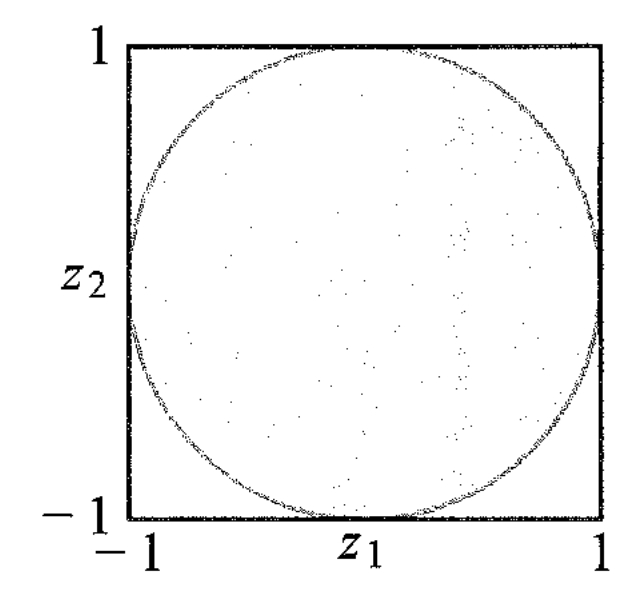
\includegraphics[width=0.28\textwidth]{ch14-fig14.3-box-muller.png}
\caption{Box-Muller 方法用于生成 Gauss 分布的随机数，为此，首先在单位圆内生成均匀分布的样本}
\label{figure:ch14-box-muller}
\end{figure}

因此，$y_{1}$ 和 $y_{2}$ 是独立的，并且每个变量都服从均值为零、方差为 $1$ 的 Gauss 分布。

\begin{proposition}[Box-Muller 方法的正确性]\label{proposition:ch14-box-muller}
设 $(z_{1},z_{2})$ 在单位圆 $\left\{(z_{1},z_{2}):z_{1}^{2}+z_{2}^{2}\leqslant 1\right\}$ 内均匀分布，$r^{2}=z_{1}^{2}+z_{2}^{2}$，$y_{1},y_{2}$ 由\eqref{align:ch14-box-muller-y1}与\eqref{align:ch14-box-muller-y2}定义。则 $y_{1},y_{2}$ 相互独立且均服从 $\mathcal{N}(0,1)$，即\eqref{align:ch14-box-muller联合}成立。
\end{proposition}

\begin{proof}
采用极坐标 $z_{1}=r\cos\theta$，$z_{2}=r\sin\theta$，其中 $r\in[0,1]$，$\theta\in[0,2\pi)$。由 $(z_{1},z_{2})$ 在单位圆上均匀分布（$p(z_{1},z_{2})=1/\pi$）及面积元 $\mathrm{d}z_{1}\mathrm{d}z_{2}=r\,\mathrm{d}r\,\mathrm{d}\theta$，$(r,\theta)$ 的联合密度为
\begin{align*}
p(r,\theta)=\frac{r}{\pi},\qquad 0\leqslant r\leqslant 1,\quad 0\leqslant\theta<2\pi,
\end{align*}
即 $\theta$ 在 $[0,2\pi)$ 上均匀、$r$ 的密度为 $2r$，且二者独立。由\eqref{align:ch14-box-muller-y1}与\eqref{align:ch14-box-muller-y2}，$y_{1}=z_{1}\varphi(r)$，$y_{2}=z_{2}\varphi(r)$，其中 $\varphi(r)=\left(-2\ln r^{2}\right)^{1/2}/r$。该变换是径向的：方向角 $\theta$ 保持不变，半径按
\begin{align*}
R\triangleq\left(y_{1}^{2}+y_{2}^{2}\right)^{1/2}=r\,\varphi(r)=\left(-2\ln r^{2}\right)^{1/2}
\end{align*}
映射，故 $r^{2}=\exp\left(-R^{2}/2\right)$，即 $r=\exp\left(-R^{2}/4\right)$。于是 $(R,\theta)$ 的联合密度为
\begin{align*}
p(R,\theta)=p(r,\theta)\left|\frac{\mathrm{d}r}{\mathrm{d}R}\right|=\frac{r}{\pi}\cdot\frac{R}{2}\exp\left(-\frac{R^{2}}{4}\right)=\frac{R}{2\pi}\exp\left(-\frac{R^{2}}{2}\right),
\end{align*}
其中用到 $\left|\mathrm{d}r/\mathrm{d}R\right|=\frac{R}{2}\exp\left(-R^{2}/4\right)$。最后换回直角坐标：由 $\mathrm{d}y_{1}\mathrm{d}y_{2}=R\,\mathrm{d}R\,\mathrm{d}\theta$，
\begin{align*}
p(y_{1},y_{2})=\frac{p(R,\theta)}{R}=\frac{1}{2\pi}\exp\left(-\frac{y_{1}^{2}+y_{2}^{2}}{2}\right)=\frac{1}{\sqrt{2\pi}}e^{-y_{1}^{2}/2}\cdot\frac{1}{\sqrt{2\pi}}e^{-y_{2}^{2}/2},
\end{align*}
它关于 $y_{1}$、$y_{2}$ 分离，故二者独立且均为标准 Gauss 分布，这正是\eqref{align:ch14-box-muller联合}。
\end{proof}

% SUPPLEMENT: parent=proposition:ch14-box-muller; kind=motivation; location=紧随其后的 remark（重构新增）
\begin{remark}（重构新增）Box-Muller 方法绕开了「对 Gauss 累积分布函数求反函数」这一障碍：Gauss 的累积分布没有初等闭式，但极坐标下的 $r^{2}$ 服从指数分布、$\theta$ 服从均匀分布，而这两者都可以用逆变换法生成，于是先产生 $(r,\theta)$ 再变回直角坐标即可。\eqref{align:ch14-box-muller-y1}中的因子 $\left(-2\ln r^{2}\right)^{1/2}/r$ 正是把半径 $r$ 拉到「Gauss 半径」的伸缩量，它不是常数，故不能把 $y_{1},y_{2}$ 看成 $z_{1},z_{2}$ 的线性变换，Jacobi行列式必须按二维变换整体计算。丢弃单位圆外的点对是必要的：若在正方形 $(-1,1)^{2}$ 上均匀取点而不筛选，则 $r$ 的密度不再是 $2r$，得到的将不是标准 Gauss 分布。
\end{remark}

如果 $y$ 服从均值为零、方差为单位方差的 Gauss 分布，那么 $\sigma y+\mu$ 将服从均值为 $\mu$、方差为 $\sigma^{2}$ 的 Gauss 分布。为了生成具有多元 Gauss 分布的向量值变量，假设多元 Gauss 分布的均值为 $\bm{\mu}$、协方差矩阵为 $\bm{\Sigma}$，我们可以利用 Cholesky 分解，其形式为 $\bm{\Sigma}=\bm{L}\bm{L}^{\mathsf{T}}$，其中 $\bm{L}$ 是一个下三角矩阵（Deisenroth, Faisal, and Ong, 2020）。然后，如果 $\bm{z}$ 是一个随机向量，其分量是独立的且具有零均值、单位方差的 Gauss 分布（见\cref{exercise:ch14-06}），那么 $\bm{y}=\bm{\mu}+\bm{L}\bm{z}$ 将具有均值为 $\bm{\mu}$、协方差矩阵为 $\bm{\Sigma}$ 的 Gauss 分布。

\begin{proposition}[多元 Gauss 分布的 Cholesky 采样]\label{proposition:ch14-cholesky}
设 $\bm{\Sigma}\in\mathbb{R}^{D\times D}$ 对称正定，$\bm{\Sigma}=\bm{L}\bm{L}^{\mathsf{T}}$ 为其 Cholesky 分解（$\bm{L}$ 为对角元为正的下三角矩阵），$\bm{z}\sim\mathcal{N}(\bm{0},\bm{I})$。则 $\bm{y}=\bm{\mu}+\bm{L}\bm{z}$ 服从 $\mathcal{N}(\bm{\mu},\bm{\Sigma})$。
\end{proposition}

\begin{proof}
由期望的线性性，$\mathbb{E}[\bm{y}]=\bm{\mu}+\bm{L}\mathbb{E}[\bm{z}]=\bm{\mu}$。由 $\operatorname{cov}[\bm{z}]=\bm{I}$ 及协方差在仿射变换下的变换规则，
\begin{align*}
\operatorname{cov}[\bm{y}]=\bm{L}\operatorname{cov}[\bm{z}]\bm{L}^{\mathsf{T}}=\bm{L}\bm{L}^{\mathsf{T}}=\bm{\Sigma}.
\end{align*}
又 $\bm{y}$ 是 Gauss 向量 $\bm{z}$ 的仿射变换，故仍为 Gauss 向量；Gauss 分布由均值与协方差唯一确定，所以 $\bm{y}\sim\mathcal{N}(\bm{\mu},\bm{\Sigma})$。
\end{proof}

% SUPPLEMENT: parent=proposition:ch14-cholesky; kind=motivation; location=紧随其后的 remark（重构新增）
\begin{remark}（重构新增）Cholesky 分解的作用是把「协方差矩阵的相关结构」翻译成「下三角线性变换」：$\bm{L}$ 的对角元给出各方向的标准差，非对角元给出方向之间的耦合，因此只需 $D$ 个独立的标准正态数就能生成具有完整协方差结构的样本，计算代价为 $O(D^{2})$。存在性由 $\bm{\Sigma}$ 正定保证：正定性等价于所有顺序主子式为正，Cholesky 分解的存在唯一性正是这一事实的构造性表述；若 $\bm{\Sigma}$ 只是半正定（例如某些方差为零），则 $\bm{L}$ 仍存在但只有半正定对角元，此时 $\bm{y}$ 落在低维仿射子空间上，不再有密度。另外，$\bm{z}$ 各分量必须独立：若 $\bm{z}$ 分量相关，$\operatorname{cov}[\bm{y}]$ 将多出交叉项，$\bm{y}$ 的协方差不再是 $\bm{\Sigma}$。
\end{remark}

显然，变换技术的成功依赖于计算所需分布的不定积分与求得其反函数的能力。这样的操作只对几种简单分布可行，因此我们必须转向替代方法，寻找更通用的策略。这里我们考虑两种替代方法：拒绝采样（rejection sampling）和重要性采样（importance sampling）。尽管这两种方法受限于单变量分布，并不能直接应用于多维的复杂问题，但它们是更通用策略的重要组成部分。

\subsection{拒绝采样}\label{subsection:ch14-拒绝采样}

拒绝采样框架允许我们从相对复杂的分布中采样，但有一定的限制条件。首先考虑单变量分布，然后考虑扩展到多维的情形。

假设我们想要从一个分布 $p(z)$ 中进行采样，该分布不属于目前为止考虑过的简单标准分布，并且直接从 $p(z)$ 中采样很困难。此外，假设我们能够轻易地计算任意给定值 $z$ 的 $\widetilde{p}(z)$，但计算结果需要乘以归一化常数 $Z_{p}$ 的倒数才能得到真实的 $p(z)$，即
\begin{align}
p(z)=\frac{1}{Z_{p}}\,\widetilde{p}(z),
\label{align:ch14-未归一化}
\end{align}
其中 $\widetilde{p}(z)$ 很容易计算，但 $Z_{p}$ 是未知的。

\begin{definition}[拒绝采样]\label{definition:ch14-拒绝采样}
设目标分布 $p(z)=\widetilde{p}(z)/Z_{p}$，其中 $\widetilde{p}$ 已知而 $Z_{p}$ 未知。设 $q(z)$ 是容易从中采样的提议分布（proposal distribution），常数 $k$ 满足对一切 $z$ 都有 $kq(z)\geqslant\widetilde{p}(z)$，称 $kq(z)$ 为比较函数。拒绝采样的每一步为：
\begin{enumerate}[(i)]
\item 从 $q(z)$ 中采样 $z_{0}$；
\item 从 $[0,kq(z_{0})]$ 上的均匀分布中采样 $u_{0}$；
\item 若 $u_{0}>\widetilde{p}(z_{0})$ 则拒绝该样本，否则保留 $z_{0}$。
\end{enumerate}
\end{definition}

% SUPPLEMENT: parent=definition:ch14-拒绝采样; kind=motivation; location=紧随其后的 remark（重构新增）
\begin{remark}（重构新增）拒绝采样的几何图像是「在比较函数曲线下均匀撒点、再按目标曲线的高度筛选」：$(z_{0},u_{0})$ 在 $kq$ 曲线下方均匀分布，若 $u_{0}\leqslant\widetilde{p}(z_{0})$ 则它落在 $\widetilde{p}$ 曲线下方，被保留的点在 $\widetilde{p}$ 下方仍然均匀，故其横坐标服从 $p$。这里有三个条件需要逐项确认。其一，$kq(z)\geqslant\widetilde{p}(z)$ 对\emph{一切} $z$ 成立，否则 $\widetilde{p}$ 的某些区域无法被覆盖，接受样本的分布会被截断；其二，$Z_{p}$ 不需要已知，因为归一化在筛选后自动完成，这是该方法相对逆变换采样的最大优势；其三，$q$ 必须有比 $\widetilde{p}$ 更重的尾部（这正是存在有限 $k$ 的含义），否则 $k$ 不存在。常数 $k$ 直接决定效率：接受概率为 $\int\widetilde{p}\,\mathrm{d}z/\left(k\int q\,\mathrm{d}z\right)=Z_{p}/k$，故 $k$ 越接近最优值 $k^{\star}=\sup_{z}\widetilde{p}(z)/q(z)$ 越好。
\end{remark}

要应用拒绝采样，我们需要一些更简单的分布 $q(z)$，它们有时称为提议分布，我们可以容易地从中抽取样本。接下来引入常数 $k$，其值的选取需要满足对于所有的 $z$ 都有 $kq(z)\geqslant\widetilde{p}(z)$。函数 $kq(z)$ 称为比较函数，\cref{figure:ch14-拒绝采样}针对一元分布的情况对它进行了说明。拒绝采样的每一步都需要生成两个随机数：先从分布 $q(z)$ 中生成一个随机数 $z_{0}$，接着从区间 $\left[0,kq(z_{0})\right]$ 上的均匀分布中生成另一个随机数 $u_{0}$。这对随机数在函数 $kq(z)$ 的曲线下具有均匀分布。最后，如果 $u_{0}>\widetilde{p}(z_{0})$，则拒绝该样本，否则保留 $z_{0}$。因此，这对随机数如果位于\cref{figure:ch14-拒绝采样}中的灰色阴影区域内，则会被拒绝。剩余的随机数对在 $\widetilde{p}(z)$ 曲线下具有均匀分布（见\cref{exercise:ch14-07}），因此相应的 $z$ 值服从我们期望的分布 $p(z)$。

\begin{figure}[htbp]
\centering
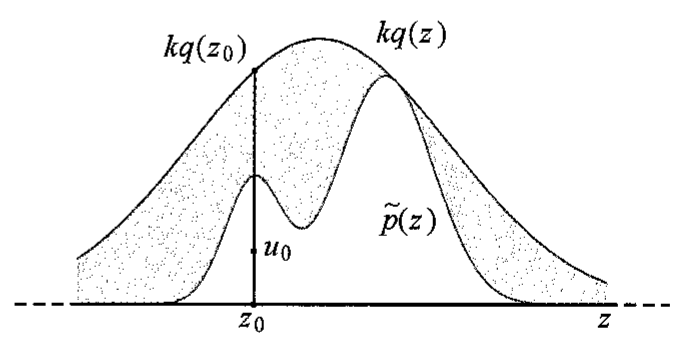
\includegraphics[width=0.5\textwidth]{ch14-fig14.4-rejection.png}
\caption{在拒绝采样中，样本是从一个简单的分布 $q(z)$ 中抽取的，并且它们如果落在未归一化分布 $\widetilde{p}(z)$ 和缩放分布 $kq(z)$ 之间的灰色区域内，则被拒绝。最终的样本是根据 $p(z)$ 分布的，$p(z)$ 是 $\widetilde{p}(z)$ 的归一化版本}
\label{figure:ch14-拒绝采样}
\end{figure}

原始的 $z$ 值是从分布 $q(z)$ 中生成的，然后这些样本以 $\widetilde{p}(z)/kq(z)$ 的概率得以接受，因此接受样本的概率由下式给出：
\begin{align}
p(\text{accept})&=\int\min\left\{\frac{\widetilde{p}(z)}{kq(z)},1\right\}q(z)\,\mathrm{d}z\nonumber\\
&=\frac{1}{k}\int\widetilde{p}(z)\,\mathrm{d}z.
\label{align:ch14-接受概率}
\end{align}

\begin{proposition}[拒绝采样的正确性]\label{proposition:ch14-拒绝采样正确性}
在\cref{definition:ch14-拒绝采样}的设定下，设 $\widetilde{p}$ 与 $q$ 均为概率密度（或均可积），$\int\widetilde{p}\,\mathrm{d}z=Z_{p}\in(0,\infty)$，且 $kq(z)\geqslant\widetilde{p}(z)$ 对一切 $z$ 成立。则被接受样本的取值服从 $p(z)=\widetilde{p}(z)/Z_{p}$，且接受概率由\eqref{align:ch14-接受概率}给出。
\end{proposition}

\begin{proof}
设事件 $A$ 表示样本被接受。给定 $z_{0}=z$ 时，$u_{0}$ 在 $\left[0,kq(z)\right]$ 上均匀分布，故
\begin{align*}
P\left(A\mid z_{0}=z\right)=P\left(u_{0}\leqslant\widetilde{p}(z)\right)=\frac{\widetilde{p}(z)}{kq(z)},
\end{align*}
这里用到 $0\leqslant\widetilde{p}(z)\leqslant kq(z)$。于是由概率的乘法规则，$z_{0}$ 落于 $\mathrm{d}z$ 且被接受的联合概率为
\begin{align*}
q(z)\,\mathrm{d}z\cdot\frac{\widetilde{p}(z)}{kq(z)}=\frac{\widetilde{p}(z)}{k}\,\mathrm{d}z,
\end{align*}
它关于 $z$ 的积分为 $Z_{p}/k$，正是 $P(A)$；因此给定 $A$ 时 $z_{0}$ 的条件密度为
\begin{align*}
p\left(z\mid A\right)=\frac{\widetilde{p}(z)/k}{Z_{p}/k}=\frac{\widetilde{p}(z)}{Z_{p}}=p(z).
\end{align*}
又 $P(A)=\int\frac{\widetilde{p}(z)}{kq(z)}q(z)\,\mathrm{d}z=\frac{1}{k}\int\widetilde{p}(z)\,\mathrm{d}z$，即\eqref{align:ch14-接受概率}。
\end{proof}

% SUPPLEMENT: parent=proposition:ch14-拒绝采样正确性; kind=motivation; location=紧随其后的 remark（重构新增）
\begin{remark}（重构新增）证明的实质是「先算联合、再条件化」：$z_{0}$ 与 $u_{0}$ 的联合分布已知，接受事件 $A$ 只是对 $u_{0}$ 的一个截断，于是 $\left(z_{0}\mid A\right)$ 的密度就是把联合密度在 $A$ 上积分后归一化。注意这里\emph{没有}要求 $\widetilde{p}$ 归一化，$Z_{p}$ 在分子分母中相消，这是拒绝采样与重要性采样共有的性质。条件 $kq\geqslant\widetilde{p}$ 保证了接受概率不超过 $1$；若某个 $z$ 使 $\widetilde{p}(z)>kq(z)$，则上式给出大于 $1$ 的「概率」，说明该 $z$ 邻域的样本永远不可能被正确筛选，接受样本的分布将缺失这一块质量。最后，接受概率 $Z_{p}/k$ 与 $z$ 无关，因此拒绝是「纯粹的浪费」，算法效率完全由 $k$ 决定。
\end{remark}

因此，这种方法拒绝的点的比例取决于未归一化分布 $\widetilde{p}(z)$ 曲线下的面积与缩放分布 $kq(z)$ 曲线下的面积的比值。由此可见，常数 $k$ 应尽可能小，同时满足对于任意 $z$，$kq(z)$ 处处都不小于 $\widetilde{p}(z)$ 的限制条件。

为了演示拒绝采样的用法，考虑从 Gamma 分布中采样的任务：
\begin{align}
\operatorname{Gam}(z\mid a,b)=\frac{b^{a}z^{a-1}\exp(-bz)}{\Gamma(a)}.
\label{align:ch14-gamma}
\end{align}

当 $a>1$，Gamma 分布具有钟形形状，如\cref{figure:ch14-gamma拒绝采样}所示。因此，合适的提议分布是 Cauchy 分布\eqref{align:ch14-cauchy分布}，因为它也是钟形的，而且我们可以使用前面讨论的变换方法从中采样。我们需要稍微扩展一下 Cauchy 分布，以确保其在任何位置的值都不小于 Gamma 分布的值。这可以通过使用 $z=b\tan y+c$ 变换均匀分布的随机变量 $y$ 来实现，这会产生服从下式分布的随机数（见\cref{exercise:ch14-08}）：
\begin{align}
q(z)=\frac{k}{1+(z-c)^{2}/b^{2}}.
\label{align:ch14-缩放cauchy}
\end{align}

\begin{figure}[htbp]
\centering
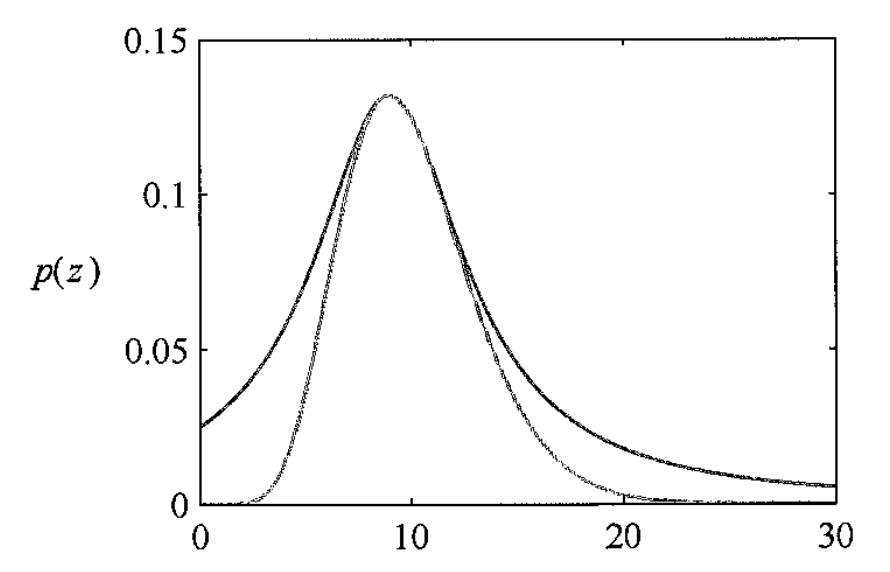
\includegraphics[width=0.42\textwidth]{ch14-fig14.5-gamma-rejection.png}
\caption{式\eqref{align:ch14-gamma}给出的 Gamma 分布为绿色曲线，缩放后的 Cauchy 提议分布为红色曲线。可以通过从 Cauchy 分布中采样，然后应用拒绝采样来获得 Gamma 分布的样本}
\label{figure:ch14-gamma拒绝采样}
\end{figure}

通过设置 $c=a-1$、$b^{2}=2a-1$，并选择尽可能小的常数 $k$ 来满足 $kq(z)\geqslant\widetilde{p}(z)$ 的要求，可以获得最小的拒绝率。最终得到的比较函数如\cref{figure:ch14-gamma拒绝采样}所示。

\begin{example}[ 用拒绝采样从 Gamma 分布中采样]\label{example:ch14-gamma拒绝采样}
设目标分布为\eqref{align:ch14-gamma}给出的 $\operatorname{Gam}(z\mid a,b)$，取提议分布为\eqref{align:ch14-缩放cauchy}，其中 $c=a-1$、$b^{2}=2a-1$。说明如何用拒绝采样得到 Gamma 分布的样本。
\end{example}

\begin{solution}（重构新增）由\eqref{align:ch14-缩放cauchy}，$q$ 是对称的钟形密度，可用 $z=c+b\tan\left(\pi\left(u-\frac{1}{2}\right)\right)$（$u\sim\mathcal{U}(0,1)$）采样，且 $q$ 的尾部按 $z^{-2}$ 衰减，比 Gamma 分布的指数尾部更重，故存在有限常数 $k$ 使 $kq\geqslant\widetilde{p}$。取
\begin{align*}
k=\sup_{z>0}\frac{\widetilde{p}(z)}{q(z)},
\end{align*}
其中 $\widetilde{p}(z)=b^{a}z^{a-1}e^{-bz}/\Gamma(a)$（$z>0$）。由于 $a>1$ 时 $\widetilde{p}$ 在 $z=(a-1)/b=c/b$ 处取极大，而 $q$ 在同一位置取极大，$k$ 由该点的比值给出（精确的最优 $k$ 需用求导或数值优化确定）。算法为：从 $q$ 采样 $z_{0}$，从 $\mathcal{U}\left(0,kq(z_{0})\right)$ 采样 $u_{0}$，若 $u_{0}\leqslant\widetilde{p}(z_{0})$ 则保留 $z_{0}$，否则拒绝。由\cref{proposition:ch14-拒绝采样正确性}，保留下来的 $z_{0}$ 服从 $\operatorname{Gam}(z\mid a,b)$，接受概率为 $Z_{p}/k$。
\end{solution}

为了使拒绝采样具有实用价值，我们要求比较函数与目标分布尽可能接近，以便将拒绝率保持在最低限度。下面看看当我们试图在高维空间中使用拒绝采样时会发生什么。我们考虑一个有点儿故意设计的问题：希望从一个均值为零、协方差为 $\sigma_{p}^{2}\bm{I}$ 的 Gauss 分布中采样（其中 $\bm{I}$ 是单位矩阵），而提议分布本身是一个均值为零、协方差为 $\sigma_{q}^{2}\bm{I}$ 的 Gauss 分布。显然，必须有 $\sigma_{q}^{2}\geqslant\sigma_{p}^{2}$ 以确保存在一个常数 $k$ 使得 $kq(z)\geqslant p(z)$。在 $D$ 维空间中，$k$ 的最优值由 $k=\left(\sigma_{q}/\sigma_{p}\right)^{D}$ 给出，参见\cref{figure:ch14-高维拒绝采样}中 $D=1$ 的情形。样本接受率将是 $p(z)$ 和 $kq(z)$ 曲线下面积的比值，因为这两个分布都是归一化的，所以结果为 $1/k$。样本接受率会随着维度的增大呈指数下降。即使 $\sigma_{q}$ 仅比 $\sigma_{p}$ 高出 $1\%$，对于 $D=1000$，接受率大约为 $1/20\,000$。

\begin{figure}[htbp]
\centering
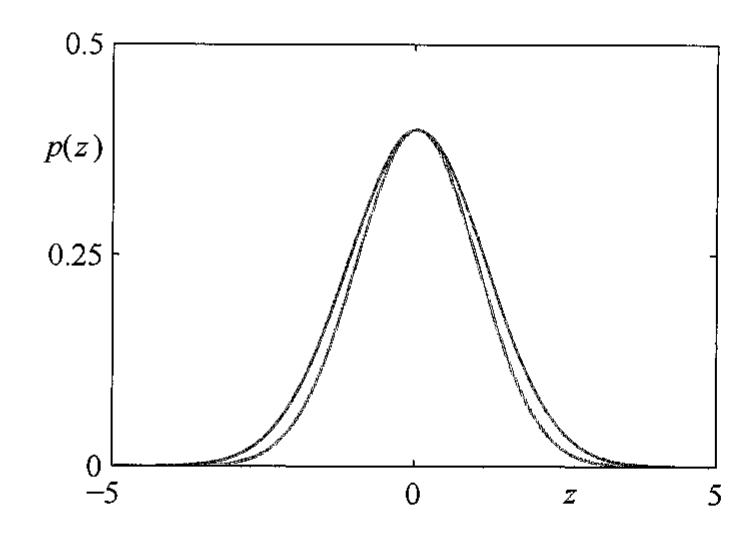
\includegraphics[width=0.42\textwidth]{ch14-fig14.7-rejection-highdim.png}
\caption{用来突出拒绝采样局限性的示例。可通过使用提议分布 $q(z)$ 进行拒绝采样，并从 Gauss 分布 $p(z)$ 中抽取样本，该分布用绿色曲线表示，其缩放版本 $kq(z)$ 用红色曲线表示，提议分布 $q(z)$ 也是 Gauss 分布}
\label{figure:ch14-高维拒绝采样}
\end{figure}

在这个例子中，比较函数接近目标分布。目标分布可能是多模态且具有尖锐峰值的，要找到一个好的提议分布和比较函数将极其困难。此外，接受率随维度呈指数下降是拒绝采样的一个普遍特性。尽管拒绝采样在一维或两维空间中可能是一种有用的技术，但它不适用于高维问题。然而，它可以作为在高维空间采样的更复杂算法中的一个子程序发挥作用。

\begin{proposition}[各向同性 Gauss 提议下的最优比较常数]\label{proposition:ch14-高维拒绝采样}
设 $p=\mathcal{N}\left(\bm{0},\sigma_{p}^{2}\bm{I}\right)$，$q=\mathcal{N}\left(\bm{0},\sigma_{q}^{2}\bm{I}\right)$，$\sigma_{q}>\sigma_{p}$，$\bm{z}\in\mathbb{R}^{D}$。则满足 $kq(\bm{z})\geqslant p(\bm{z})$ 对一切 $\bm{z}$ 成立的最小常数为
\begin{align}
k=\left(\frac{\sigma_{q}}{\sigma_{p}}\right)^{D},
\label{align:ch14-高维比较常数}
\end{align}
相应的接受概率为 $1/k=\left(\sigma_{p}/\sigma_{q}\right)^{D}$。
\end{proposition}

\begin{proof}
两个密度的比值为
\begin{align*}
\frac{p(\bm{z})}{q(\bm{z})}=\left(\frac{\sigma_{q}}{\sigma_{p}}\right)^{D}\exp\left(-\frac{1}{2}\left(\frac{1}{\sigma_{p}^{2}}-\frac{1}{\sigma_{q}^{2}}\right)\lVert\bm{z}\rVert^{2}\right),
\end{align*}
由于 $\sigma_{q}>\sigma_{p}$，指数上的系数 $\frac{1}{\sigma_{p}^{2}}-\frac{1}{\sigma_{q}^{2}}>0$，故该比值在 $\bm{z}=\bm{0}$ 处取最大值，最大值即\eqref{align:ch14-高维比较常数}。取 $k$ 等于该最大值时 $kq\geqslant p$ 处处成立，且任何更小的 $k$ 都会在 $\bm{z}=\bm{0}$ 处失效，故它是最小常数。接受概率由\eqref{align:ch14-接受概率}，因 $p,q$ 均已归一化，得 $1/k$。
\end{proof}

% SUPPLEMENT: parent=proposition:ch14-高维拒绝采样; kind=motivation; location=紧随其后的 remark（重构新增）
\begin{remark}（重构新增）本命题定量地说明了「维数灾难」在拒绝采样中的具体形态：$k$ 是每维比值 $\sigma_{q}/\sigma_{p}$ 的 $D$ 次幂，因此即使单维上提议分布只比目标分布「胖」$1\%$，在 $D=1000$ 维时 $k\approx1.01^{1000}\approx2\times10^{4}$，接受率降至约 $1/20\,000$。这里 $k$ 的最优性依赖于两个分布同为各向同性 Gauss：此时密度比只通过 $\lVert\bm{z}\rVert^{2}$ 依赖 $\bm{z}$，最大值在原点取得；若目标分布是多模态或有尖峰，密度比的最大值会出现在某个难以预知的点，$k$ 既难计算又往往极大。条件 $\sigma_{q}>\sigma_{p}$ 是必要的：若 $\sigma_{q}\leqslant\sigma_{p}$，则 $p/q$ 在 $\lVert\bm{z}\rVert\to\infty$ 时无界，不存在有限 $k$，这正是「提议分布必须有更重的尾」的一维特例。命题也解释了为什么拒绝采样在高维只能作为子程序：把维度拆成若干低维块分别处理，才能把 $k$ 的指数增长控制在可接受范围内。
\end{remark}

\subsection{适应性拒绝采样}\label{subsection:ch14-适应性拒绝采样}

许多时候，我们希望使用拒绝采样方法却很难确定包络分布 $q(z)$ 的合适解析形式。一种替代方法是基于分布 $\widetilde{p}(z)$ 的测量值构造包络函数（Gilks and Wild, 1992）。当 $p(z)$ 是对数凹函数时，即 $\ln p(z)$ 的导数是 $z$ 的非增函数时，构造合适的包络函数尤其简单。构造的包络函数的说明见\cref{figure:ch14-自适应包络}。

\begin{definition}[对数凹函数]\label{definition:ch14-对数凹}
设 $p(z)>0$ 定义在区间 $I$ 上。若 $\ln p(z)$ 是凹函数，即对任意 $z_{1},z_{2}\in I$ 与 $t\in[0,1]$ 有
\begin{align*}
\ln p\left(tz_{1}+(1-t)z_{2}\right)\geqslant t\ln p(z_{1})+(1-t)\ln p(z_{2}),
\end{align*}
则称 $p$ 是对数凹（log-concave）的。若 $\ln p$ 可微，则等价于 $\left(\ln p\right)'$ 在 $I$ 上非增。
\end{definition}

% SUPPLEMENT: parent=definition:ch14-对数凹; kind=motivation; location=紧随其后的 remark（重构新增）
\begin{remark}（重构新增）对数凹性是适应性拒绝采样能够「自动构造包络」的关键：$\ln p$ 凹意味着它的图像位于任意切线的下方，于是取若干网格点处的切线、再取这些切线的逐点最大值，就得到一个\emph{分段线性}的上界，其指数即为一个分段指数的包络密度，且该包络可以精确地归一化与采样。若 $p$ 不是对数凹的，切线可能落在 $\ln p$ 的下方，包络不再成立，算法必须加入 Metropolis-Hastings 修正（见\cref{subsection:ch14-Metropolis-Hastings}）。常见的对数凹分布包括 Gauss、指数、Gamma（$a\geqslant1$）、Beta（参数均 $\geqslant1$）等；混合分布通常不是对数凹的，因为 $\ln\left(\pi_{1}p_{1}+\pi_{2}p_{2}\right)$ 一般不是凹函数。注意定义只涉及 $\ln p$ 而不涉及 $p$ 本身：$p$ 本身不必是凹的（例如 Gauss 密度在均值附近是凸的）。
\end{remark}

首先，在一些初始网格点上计算 $\ln\widetilde{p}(z)$ 及其梯度，然后利用得到的切线交点来构造包络函数。接下来，从包络分布中抽取一个样本值（见\cref{exercise:ch14-10}）。这一步很简单，因为包络分布的对数是一系列线性函数，因此包络分布本身是由以下形式的分段指数分布构成的：
\begin{align}
q(z)=k_{j}\lambda_{j}\exp\left\{-\lambda_{j}\left(z-z_{j-1}\right)\right\},\qquad z_{j-1}<z\leqslant z_{j}.
\label{align:ch14-分段指数包络}
\end{align}

\begin{figure}[htbp]
\centering
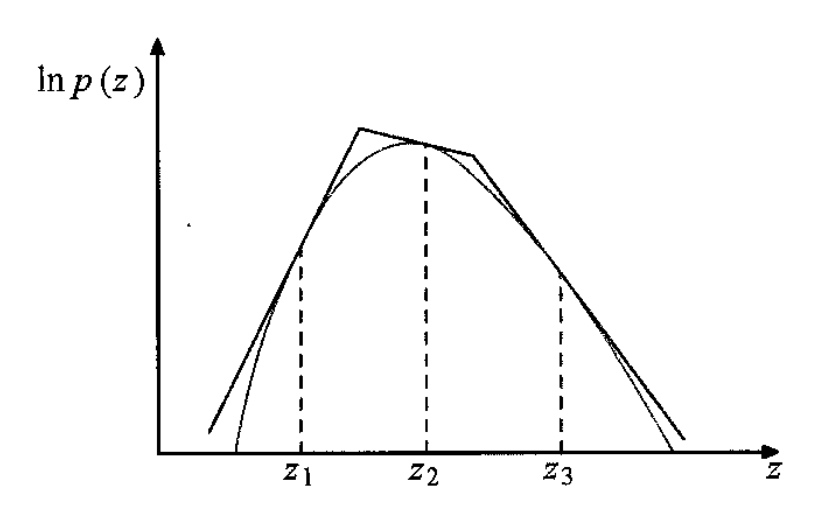
\includegraphics[width=0.42\textwidth]{ch14-fig14.6-adaptive-envelope.png}
\caption{在拒绝采样中，如果一个分布是对数凹的，则可以使用我们在一组网格点计算得到的切线来构造一个包络函数。如果一个样本被拒绝，就将它添加到网格点集合中，并用于完善包络分布}
\label{figure:ch14-自适应包络}
\end{figure}

一旦抽取了一个样本，就可以应用常规的拒绝标准。样本如果被接受，它将是期望分布的一个抽取。样本如果被拒绝，它就被纳入网格点集合中，用于计算新的切线，并由此完善包络函数。随着网格点数量的增加，包络函数会越来越逼近期望分布 $p(z)$，并且样本被拒绝的概率就会降低。

Gilks 提出了旨在避免计算导数的自适应拒绝采样（Gilks, 1992）。自适应拒绝采样框架也可以扩展到非对数凹分布，只需要在每个拒绝采样步骤之后跟随一个 Metropolis-Hastings 步骤（将在\cref{subsection:ch14-Metropolis-Hastings}中讨论），从而产生自适应拒绝 Metropolis 采样（Gilks, Best, and Tan, 1995）。

\subsection{重要性采样}\label{subsection:ch14-重要性采样}

我们希望从复杂概率分布中进行采样的一个原因是为了计算形如\eqref{align:ch14-期望定义}的期望。重要性采样技术提供了一个直接近似期望的框架，但它本身并不提供从分布 $p(\bm{z})$ 中抽取样本的方法。

式\eqref{align:ch14-mc估计}给出的有限和近似期望值，依赖于能够从分布 $p(\bm{z})$ 中抽取样本。然而，假设直接从 $p(\bm{z})$ 中采样是不现实的，但对于任意给定的 $\bm{z}$ 值，我们能够容易地计算出 $\widetilde{p}(\bm{z})$ 的值。一种简单的计算期望方法是将 $\bm{z}$ 空间离散化为均匀网格，并将期望表示成求和的形式：
\begin{align}
\mathbb{E}[f]\approx\sum_{l=1}^{L}p\!\left(\bm{z}^{(l)}\right)f\!\left(\bm{z}^{(l)}\right).
\label{align:ch14-离散网格}
\end{align}

这种方法的一个明显问题是，求和项的数量会随着 $\bm{z}$ 的维度的增加呈指数增长。此外，正如我们已经注意到的，我们感兴趣的概率分布通常会将它们的大部分概率密度限制在 $\bm{z}$ 空间的相对较小的区域内，所以在高维问题中，均匀采样将非常低效，因为只有很少一部分样本会对求和做出显著贡献。我们真正希望的是在 $p(\bm{z})$ 较大的区域，或理想情况下，从 $p(\bm{z})f(\bm{z})$ 较大的区域中选择样本点。

\begin{figure}[htbp]
\centering
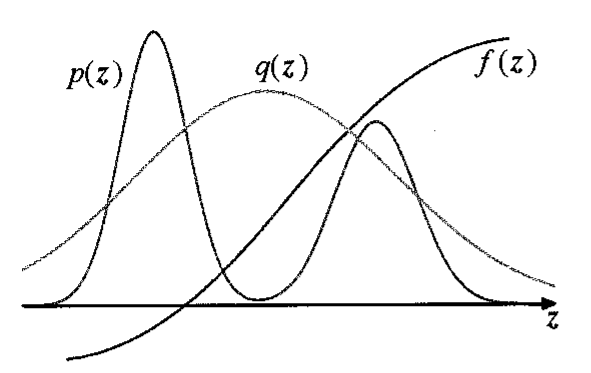
\includegraphics[width=0.45\textwidth]{ch14-fig14.8-importance.png}
\caption{重要性采样解决了这样一个问题：当我们很难直接从分布 $p(z)$ 中采样时，如何计算函数 $f(z)$ 关于该分布的期望。此方法从更易采样的分布 $q(z)$ 中抽取样本 $\left\{z^{(l)}\right\}$，并且在求和计算中为每个样本项赋予权重 $p\left(z^{(l)}\right)/q\left(z^{(l)}\right)$}
\label{figure:ch14-重要性采样}
\end{figure}

与拒绝采样一样，重要性采样也基于易于抽取样本的提议分布 $q(\bm{z})$，如\cref{figure:ch14-重要性采样}所示。我们可以利用从 $q(\bm{z})$ 中抽取的样本集 $\left\{\bm{z}^{(l)}\right\}$，将期望表达为样本上的有限和形式：
\begin{align}
\mathbb{E}[f]&=\int f(\bm{z})p(\bm{z})\,\mathrm{d}\bm{z}\nonumber\\
&=\int f(\bm{z})\frac{p(\bm{z})}{q(\bm{z})}q(\bm{z})\,\mathrm{d}\bm{z}\nonumber\\
&\approx\frac{1}{L}\sum_{l=1}^{L}\frac{p\!\left(\bm{z}^{(l)}\right)}{q\!\left(\bm{z}^{(l)}\right)}f\!\left(\bm{z}^{(l)}\right).
\label{align:ch14-重要性采样}
\end{align}

\begin{definition}[重要性权重]\label{definition:ch14-重要性权重}
在重要性采样中，称
\begin{align*}
r_{l}=\frac{p\!\left(\bm{z}^{(l)}\right)}{q\!\left(\bm{z}^{(l)}\right)}
\end{align*}
为样本 $\bm{z}^{(l)}$ 的重要性权重（importance weights），其中 $\bm{z}^{(l)}\sim q$，$\widetilde{p}$ 为与 $p$ 成比例的未归一化分布。
\end{definition}

% SUPPLEMENT: parent=definition:ch14-重要性权重; kind=motivation; location=紧随其后的 remark（重构新增）
\begin{remark}（重构新增）重要性权重的动机是「换测度」：$\mathbb{E}_{p}[f]=\int f\,p\,\mathrm{d}\bm{z}=\int f\frac{p}{q}q\,\mathrm{d}\bm{z}=\mathbb{E}_{q}\left[f\frac{p}{q}\right]$，于是只要能从 $q$ 采样，就可以通过对 $f$ 乘上权重 $p/q$ 来计算 $p$ 下的期望，权重正好纠正了「从错误分布采样」引入的偏差。定义中的 $\widetilde{p}$ 不必归一化：若用 $p=\widetilde{p}/Z_{p}$ 与 $q=\widetilde{q}/Z_{q}$，则常数之比会在归一化权重中相消（见\eqref{align:ch14-归一化权重}）。使用权重的前提是 $q(\bm{z})>0$ 在 $p(\bm{z})f(\bm{z})\neq0$ 的区域成立，否则该区域被系统性漏掉，权重再大也无法补救；这是重要性采样最容易被忽视的条件，也是它与拒绝采样共享的「支撑集覆盖」要求。
\end{remark}

量 $r_{l}=p\!\left(\bm{z}^{(l)}\right)/q\!\left(\bm{z}^{(l)}\right)$ 称为重要性权重，用于纠正从错误分布中采样而引入的偏差。请注意，与拒绝采样不同，这里生成的所有样本都会被保留。

通常分布 $p(\bm{z})$ 的计算只能达到一个归一化常数的精度，所以 $p(\bm{z})=\widetilde{p}(\bm{z})/Z_{p}$，其中 $\widetilde{p}(\bm{z})$ 可以轻易计算出来，而 $Z_{p}$ 是未知的。类似地，我们可能希望使用的重要性采样分布 $q(\bm{z})=\widetilde{q}(\bm{z})/Z_{q}$ 也具有同样的性质：
\begin{align}
\mathbb{E}[f]&=\int f(\bm{z})p(\bm{z})\,\mathrm{d}\bm{z}\nonumber\\
&=\frac{Z_{q}}{Z_{p}}\int f(\bm{z})\frac{\widetilde{p}(\bm{z})}{\widetilde{q}(\bm{z})}q(\bm{z})\,\mathrm{d}\bm{z}\nonumber\\
&\approx\frac{Z_{q}}{Z_{p}}\frac{1}{L}\sum_{l=1}^{L}\tilde{r}_{l}f\!\left(\bm{z}^{(l)}\right),
\label{align:ch14-重要性采样归一化}
\end{align}
其中 $\tilde{r}_{l}=\widetilde{p}\!\left(\bm{z}^{(l)}\right)/\widetilde{q}\!\left(\bm{z}^{(l)}\right)$。我们可以使用相同的样本集来计算比值 $Z_{p}/Z_{q}$，结果为
\begin{align}
\frac{Z_{p}}{Z_{q}}&=\frac{1}{Z_{q}}\int\widetilde{p}(\bm{z})\,\mathrm{d}\bm{z}=\int\frac{\widetilde{p}(\bm{z})}{\widetilde{q}(\bm{z})}q(\bm{z})\,\mathrm{d}\bm{z}\nonumber\\
&\approx\frac{1}{L}\sum_{l=1}^{L}\tilde{r}_{l}.
\label{align:ch14-归一化常数比}
\end{align}

因此，\eqref{align:ch14-重要性采样归一化}中的期望可用加权和来表示：
\begin{align}
\mathbb{E}[f]\approx\sum_{l=1}^{L}w_{l}f\!\left(\bm{z}^{(l)}\right),
\label{align:ch14-加权和}
\end{align}
其中
\begin{align}
w_{l}=\frac{\tilde{r}_{l}}{\sum_{m}\tilde{r}_{m}}=\frac{\widetilde{p}\!\left(\bm{z}^{(l)}\right)/q\!\left(\bm{z}^{(l)}\right)}{\sum_{m}\widetilde{p}\!\left(\bm{z}^{(m)}\right)/q\!\left(\bm{z}^{(m)}\right)}.
\label{align:ch14-归一化权重}
\end{align}
请注意，$\left\{w_{l}\right\}$ 都是非负数且和为 $1$。

\begin{proposition}[重要性采样估计的无偏性]\label{proposition:ch14-重要性采样无偏}
设 $\bm{z}^{(l)}\sim q$ 独立同分布，$q(\bm{z})>0$ 在 $\left\{\bm{z}:p(\bm{z})f(\bm{z})\neq0\right\}$ 上成立，且 $\mathbb{E}_{q}\left[\left|f(\bm{z})\frac{p(\bm{z})}{q(\bm{z})}\right|\right]<\infty$。则由\eqref{align:ch14-重要性采样}定义的估计量
\begin{align*}
\overline{f}_{q}=\frac{1}{L}\sum_{l=1}^{L}\frac{p\!\left(\bm{z}^{(l)}\right)}{q\!\left(\bm{z}^{(l)}\right)}f\!\left(\bm{z}^{(l)}\right)
\end{align*}
是 $\mathbb{E}_{p}[f]$ 的无偏估计。
\end{proposition}

\begin{proof}
对每一项取关于 $q$ 的期望，并利用 $p$ 为归一化密度：
\begin{align*}
\mathbb{E}_{q}\left[\frac{p(\bm{z})}{q(\bm{z})}f(\bm{z})\right]=\int\frac{p(\bm{z})}{q(\bm{z})}f(\bm{z})\,q(\bm{z})\,\mathrm{d}\bm{z}=\int p(\bm{z})f(\bm{z})\,\mathrm{d}\bm{z}=\mathbb{E}_{p}[f],
\end{align*}
这里用到 $q(\bm{z})>0$ 在 $p(\bm{z})f(\bm{z})\neq0$ 处成立，从而被积函数关于 $q\,\mathrm{d}\bm{z}$ 可积。由期望的线性性，$\mathbb{E}_{q}\left[\overline{f}_{q}\right]=\mathbb{E}_{p}[f]$。对自归一化形式\eqref{align:ch14-重要性采样归一化}，由大数定律，
\begin{align*}
\frac{1}{L}\sum_{l=1}^{L}\tilde{r}_{l}\longrightarrow\frac{Z_{p}}{Z_{q}},
\end{align*}
故加权和几乎必然收敛到 $\mathbb{E}_{p}[f]$；但它是两个随机量之比，一般只有 $O(1/L)$ 的偏差。
\end{proof}

% SUPPLEMENT: parent=proposition:ch14-重要性采样无偏; kind=motivation; location=紧随其后的 remark（重构新增）
\begin{remark}（重构新增）无偏性只对\emph{未归一化}的形式\eqref{align:ch14-重要性采样}成立；一旦使用自归一化权重\eqref{align:ch14-归一化权重}，估计量变成两个随机量之比，其期望一般不等于 $\mathbb{E}_{p}[f]$，偏差为 $O(1/L)$，但它是相合的（$L\to\infty$ 时收敛），实践中因不需要 $Z_{p}$ 而更常用。条件 $\mathbb{E}_{q}\left[\left|f\,p/q\right|\right]<\infty$ 比\cref{proposition:ch14-mc无偏性}中的条件更强：即使 $f$ 有界，若 $q$ 的尾部比 $p$ 轻，则 $p/q$ 无界，方差可能无穷大，估计量虽无偏却极不稳定。这正是下文强调「$q$ 在 $p$ 显著的区域不能太小」的原因，也是有效样本量
\begin{align*}
\mathrm{ESS}=\frac{\left(\sum_{l}w_{l}\right)^{2}}{\sum_{l}w_{l}^{2}}
\end{align*}
被用来诊断权重退化的原因。
\end{remark}

与拒绝采样一样，重要性采样的成功严重依赖于采样分布 $q(\bm{z})$ 与目标分布 $p(\bm{z})$ 的匹配程度。如果 $p(\bm{z})f(\bm{z})$ 变化剧烈并且其大部分概率密度集中在 $\bm{z}$ 空间的相对较小的区域内（这种情况很常见），则一组重要性权重 $\left\{r_{l}\right\}$ 可能会受少数几个较大权重的支配，剩余的权重则相对无关紧要。因此，有效样本的数量可能比表面上的样本数 $L$ 少得多。如果没有任何样本落在 $p(\bm{z})f(\bm{z})$ 较大的区域内，问题将更为严重。在那种情况下，即使 $r_{l}$ 和 $r_{l}f\!\left(\bm{z}^{(l)}\right)$ 的表面方差可能很小，对期望的估计也可能产生严重错误。因此，重要性采样的一个主要缺点是，它可能产生任意错误的结果，并且没有诊断指标。这也突出了采样分布 $q(\bm{z})$ 的一个关键要求，即在 $p(\bm{z})$ 可能显著的区域内，它的值不应该太小或为零。

\subsection{采样-重要性-重采样}\label{subsection:ch14-采样重要性重采样}

\cref{subsection:ch14-拒绝采样}讨论的拒绝采样部分地依赖于成功确定一个适当的 $k$ 值。对于分布 $p(z)$ 和 $q(z)$ 的各种组合，想要确定一个适当的 $k$ 值是不切实际的，因为当 $k$ 值大到能保证目标分布被包络的时候，对应的样本接受率会小到没有实用价值。

与拒绝采样一样，采样-重要性-重采样方案也使用一个采样分布 $q(z)$，但避免了确定 $k$ 值的要求。该方案分两个阶段。在第一阶段，从 $q(z)$ 中抽取 $L$ 个样本 $z^{(1)},\cdots,z^{(L)}$。然后在第二阶段，使用\eqref{align:ch14-归一化权重}构建权重 $\left(w_{1},\cdots,w_{L}\right)$。最后从离散分布 $\left(z^{(1)},\cdots,z^{(L)}\right)$ 中抽取第二组 $L$ 个样本，其被抽中的概率由权重 $\left(w_{1},\cdots,w_{L}\right)$ 给出。

得到的 $L$ 个样本只是近似按照 $p(z)$ 分布的，但随着 $L$ 趋于无穷大，该分布将变得正确。为了理解这一点，考虑单变量情况，并注意重采样值的累积分布由下式给出：
\begin{align}
p(z<a)=\sum_{l}w_{l}\,\mathbb{I}\!\left(z^{(l)}\leqslant a\right)\simeq\int\mathbb{I}(z\leqslant a)\,p(z)\,\mathrm{d}z,
\label{align:ch14-重采样累积分布}
\end{align}
其中 $\mathbb{I}(\cdot)$ 是指示函数（如果其参数为真，则函数值为 $1$，否则为 $0$）。使 $L$ 趋于无穷大，并假设分布的适当的正则性，我们就可以用根据原始采样分布 $q(z)$ 加权的积分来替换求和：
\begin{align}
p(z<a)\simeq\int\mathbb{I}(z\leqslant a)\frac{\widetilde{p}(z)}{q(z)}q(z)\,\mathrm{d}z.
\label{align:ch14-重采样极限}
\end{align}
这就是 $p(z)$ 的累积分布函数。同样，我们可以看到 $p(z)$ 的归一化并不是必需的。

\begin{proposition}[重采样分布的一致性]\label{proposition:ch14-重采样一致性}
设 $z^{(l)}\sim q$ 独立同分布，权重由\eqref{align:ch14-归一化权重}给出，且 $q(z)>0$ 在 $\left\{z:p(z)\neq0\right\}$ 上成立。则对任意 $a$，当 $L\to\infty$ 时\eqref{align:ch14-重采样累积分布}的右端依概率收敛于 $p(z<a)=\int_{-\infty}^{a}p(z)\,\mathrm{d}z$。
\end{proposition}

\begin{proof}
把\eqref{align:ch14-重采样累积分布}中的 $w_{l}$ 写成自归一化形式，并分子分母同乘 $L$：
\begin{align*}
\sum_{l}w_{l}\mathbb{I}\!\left(z^{(l)}\leqslant a\right)=\frac{\frac{1}{L}\sum_{l}\tilde{r}_{l}\mathbb{I}\!\left(z^{(l)}\leqslant a\right)}{\frac{1}{L}\sum_{l}\tilde{r}_{l}}.
\end{align*}
由大数定律，分母收敛于 $\mathbb{E}_{q}\left[\tilde{r}\right]=Z_{p}/Z_{q}$，分子收敛于
\begin{align*}
\mathbb{E}_{q}\left[\tilde{r}\,\mathbb{I}(z\leqslant a)\right]=\int\frac{\widetilde{p}(z)}{\widetilde{q}(z)}\mathbb{I}(z\leqslant a)\,q(z)\,\mathrm{d}z=\frac{Z_{p}}{Z_{q}}\int\mathbb{I}(z\leqslant a)p(z)\,\mathrm{d}z.
\end{align*}
两式相除即得 $p(z<a)$。这里用到 $\mathbb{I}$ 有界，从而上述期望有限，大数定律适用。
\end{proof}

% SUPPLEMENT: parent=proposition:ch14-重采样一致性; kind=motivation; location=紧随其后的 remark（重构新增）
\begin{remark}（重构新增）重采样的实质是「用样本经验分布 $\sum_{l}w_{l}\delta_{z^{(l)}}$ 逼近 $p$」：它先允许用任意 $q$ 生成候选点，再用权重把候选点重新分配到正确的概率质量上，因此不需要比较函数 $k$，也不会像拒绝采样那样丢弃样本。代价是重采样引入了额外的随机性：同一批 $L$ 个候选点经重采样后可能出现重复值，样本之间不再独立，且当权重高度集中时（少数 $w_{l}$ 接近 $1$），重采样后的样本几乎全部来自少数几个候选点，多样性急剧下降——这正是粒子滤波中「样本贫化」现象的来源。命题中的一致性只保证 $L\to\infty$ 时的极限正确，有限 $L$ 的偏差与权重的方差成正比，故实践中仍需监控有效样本量。当 $q=p$ 时所有 $w_{l}=1/L$，重采样等价于对原样本再做一次均匀抽样，分布不变。
\end{remark}

对于有限值 $L$ 和给定的初始样本集，重采样值只能近似地从目标分布中抽取。与拒绝采样一样，随着采样分布 $q(z)$ 更接近目标分布 $p(z)$，近似结果的效果也会越来越好。当 $q(z)=p(z)$ 时，初始样本 $\left\{z^{(1)},\cdots,z^{(L)}\right\}$ 具有目标分布，且权重 $w_{l}=1/L$，因此重采样值也具有目标分布。

如果需要关于分布 $p(z)$ 的矩，则可以直接使用原始样本连同权重来计算，因为
\begin{align}
\mathbb{E}[f(z)]=\int f(z)\,p(z)\,\mathrm{d}z.
\label{align:ch14-重采样矩}
\end{align}

\end{document}
